%% 
%% Copyright 2007, 2008, 2009 Elsevier Ltd
%% 
%% This file is part of the 'Elsarticle Bundle'.
%% ---------------------------------------------
%% 
%% It may be distributed under the conditions of the LaTeX Project Public
%% License, either version 1.2 of this license or (at your option) any
%% later version.  The latest version of this license is in
%%    http://www.latex-project.org/lppl.txt
%% and version 1.2 or later is part of all distributions of LaTeX
%% version 1999/12/01 or later.
%% 
%% The list of all files belonging to the 'Elsarticle Bundle' is
%% given in the file `manifest.txt'.
%% 
%% Template article for Elsevier's document class `elsarticle'
%% with harvard style bibliographic references
%% SP 2008/03/01

\documentclass[preprint,12pt,authoryear]{elsarticle}

%% Use the option review to obtain double line spacing
%% \documentclass[authoryear,preprint,review,12pt]{elsarticle}

%% Use the options 1p,twocolumn; 3p; 3p,twocolumn; 5p; or 5p,twocolumn
%% for a journal layout:
%% \documentclass[final,1p,times,authoryear]{elsarticle}
%% \documentclass[final,1p,times,twocolumn,authoryear]{elsarticle}
%% \documentclass[final,3p,times,authoryear]{elsarticle}
%% \documentclass[final,3p,times,twocolumn,authoryear]{elsarticle}
%% \documentclass[final,5p,times,authoryear]{elsarticle}
%% \documentclass[final,5p,times,twocolumn,authoryear]{elsarticle}

%% For including figures, graphicx.sty has been loaded in
%% elsarticle.cls. If you prefer to use the old commands
%% please give \usepackage{epsfig}

%% The amssymb package provides various useful mathematical symbols
\usepackage{amssymb}
\usepackage{amsmath}
\usepackage{color, soul}
\usepackage{url}
%% The amsthm package provides extended theorem environments
%% \usepackage{amsthm}

%% The lineno packages adds line numbers. Start line numbering with
%% \begin{linenumbers}, end it with \end{linenumbers}. Or switch it on
%% for the whole article with \linenumbers.
\usepackage{lineno}

%% Block of code for fixing corresponding author bug 
%% in elsarticle template... Don't really understand it
\makeatletter
\def\@author#1{\g@addto@macro\elsauthors{\normalsize%
    \def\baselinestretch{1}%
    \upshape\authorsep#1\unskip\textsuperscript{%
      \ifx\@fnmark\@empty\else\unskip\sep\@fnmark\let\sep=,\fi
      \ifx\@corref\@empty\else\unskip\sep\@corref\let\sep=,\fi
      }%
    \def\authorsep{\unskip,\space}%
    \global\let\@fnmark\@empty
    \global\let\@corref\@empty  %% Added
    \global\let\sep\@empty}%
    \@eadauthor={#1}
}
\makeatother
%% End block of weird code


%% Command for bold Greek symbols
\newcommand{\mitbf}[1]{\hbox{\mathversion{bold}$#1$}}

\journal{Earth and Planetary Science Letters}

\begin{document}

\begin{frontmatter}

%% Title, authors and addresses

%% use the tnoteref command within \title for footnotes;
%% use the tnotetext command for theassociated footnote;
%% use the fnref command within \author or \address for footnotes;
%% use the fntext command for theassociated footnote;
%% use the corref command within \author for corresponding author footnotes;
%% use the cortext command for theassociated footnote;
%% use the ead command for the email address,
%% and the form \ead[url] for the home page:
%% \title{Title\tnoteref{label1}}
%% \tnotetext[label1]{}
%% \author{Name\corref{cor1}\fnref{label2}}
%% \ead{email address}
%% \ead[url]{home page}
%% \fntext[label2]{}
%% \cortext[cor1]{}
%% \address{Address\fnref{label3}}
%% \fntext[label3]{}

\title{Bayesian inversion for paleomagnetic reconstruction and plate kinematics}

%% use optional labels to link authors explicitly to addresses:
%% \author[label1,label2]{}
%% \address[label1]{}
%% \address[label2]{}

\author{Ian Rose\corref{cor1}\fnref{ref1}}
\author{Bruce Buffett\fnref{ref1}}
\author{Nicholas Swanson-Hysell\fnref{ref1}}

\fntext[ref1]{University of California, Berkeley}
\cortext[cor1]{Corresponding author, \url{ian.rose@berkeley.edu}}

\address{}

\begin{abstract}
%% Text of abstract

\end{abstract}

\begin{keyword}
%% keywords here, in the form: keyword \sep keyword

%% PACS codes here, in the form: \PACS code \sep code

%% MSC codes here, in the form: \MSC code \sep code
%% or \MSC[2008] code \sep code (2000 is the default)

\end{keyword}

\end{frontmatter}

\linenumbers

%% main text
\section{Introduction}
\label{sec:introduction}

Plate tectonics is the motion of near-rigid blocks of lithosphere across the surface of Earth, 
separated by narrow regions of deformation in spreading centers, transform faults, and subduction zones.
The overall rigidity of plate motions means that the motion of a great majority of Earth's surface
can be described by a set of Euler poles which specify the position and magnitude of the rotation axis for a
given plate \citep[cf.][]{cox2009plate}. The motion of individual points on a plate undergoing
a rigid rotation is described by small circles.

Euler poles are ubiquitous in describing current plate motions 
\citep[e.g.][]{demets1990current, argus2011geologically} due to their simplicity and compactness.
Furthermore, there are good reasons to think that plate motions remain constant, or approximately
so, over millions to tens of millions of years. This is most dramatically seen in the shape
of oceanic fracture zones and in hotspot tracks across the lithosphere. These features
form gently curving arcs over large portions of Earth's surface which are well described by small
circles, consistent with finite Euler rotations of the plate for an extended period of time.
As such, the combination of an Euler pole plus a time interval through which it rotates 
(often called a ``stage pole'') is a convenient description of plate motions through Earth history.

The stage pole description of plate motions is therefore a convenient way of reconstructing
plate tectonic history, and is widely used in both continental reconstruction 
\citep[e.g.][]{boyden2011next} and in geodynamical
modeling \citep[e.g.][]{mcnamara2005thermochemical, bull2014effect, rudolph2014history}.
Most reconstructions of plate motions rely heavily on fitting Euler pole rotations
to oceanic fracture zones, hotspot tracks, seafloor magnetic isochrons,
and, to a lesser extent, paleomagnetic data \citep{muller1993revised, seton2012global}.
However, as we look further back in Earth history, the records on which these
plate tectonic reconstructions rely largely disappear due to the continual
subduction of oceanic lithosphere. Before $\sim$200 Ma there is no oceanic record,
and the paleomagnetic record from continental rocks is all that remains.

It is more challenging to reconstruct past plate motions from the paleomagnetic
record for a number of reasons, including 
(1) the data is usually sparser and with larger uncertainties,
(2) traditional paleomagnetic analysis has no way of constraining paleolongitude, and
(3) many paleomagnetic poles have poor age control.

\citet{gordon1984paleomagnetic} noted that apparent polar wander paths (APWPs) have 
arcing trajectories similar to fracture zones and hotspot tracks, which is
to be expected if similar tectonic processes are responsible for creating them.
They therefore suggested fitting small circles to paleomagnetic poles tracks,
which would furnish Euler poles for the plate in question for that time period.
This model for understaning APWPs, called paleomagnetic Euler pole (PEP) analysis,
 had the attractive feature of providing a complete description of the plate motion, 
including paleolongitudinal changes and speeds. 
However, it had the drawback of being somewhat difficult to calculate,
uncertainties in the fit were not easily computed, 
and it did not incorporate age uncertainties. 
A rigorous treatment of the uncertainties requires significant computational effort.
With a few exceptions \citep{beck1989paleomagnetism, tarling1996palaeomagnetic, bryan1986rotation, beck2003absolute, smirnov2010co} 
PEP analysis has not seen wide adoption.

Herein we extend paleomagnetic Euler pole analysis by placing it within
a Bayesian statistical framework, and demonstrate how to invert for PEPs
using Markov Chain Monte Carlo (MCMC) methods. This framework has the advantage
of naturally incorporating uncertainties in the paleomagnetic pole positions,
as well as widely disparate age uncertainties that commonly occur in APWPs.
The resulting stage poles for which we invert is not a single answer, but is instead
a distribution of possible answers, furnishing uncertainties as part of the solution process.

The paper is organized as follows: in Section~\ref{sec:apwp} we review different
approaches for interpreting APWPs. In Section~\ref{sec:bayesian_inversion} we
describe the formalism of Bayesian inversions and Markov Chain Monte Carlo methods.
In Section~\ref{sec:model} we describe the statistical model which we will be inverting.
In Section~\ref{sec:example_inversion} we demonstrate the inversion on several
synthetic data sets. In Sections~\ref{sec:australia} and~\ref{sec:keweenawan}
we show examples using real paleomagnetic data from Australia and Laurentia,
including interpretations of plate speeds.

\section{Interpretation of APW paths}
\label{sec:apwp}
\begin{figure*}
%%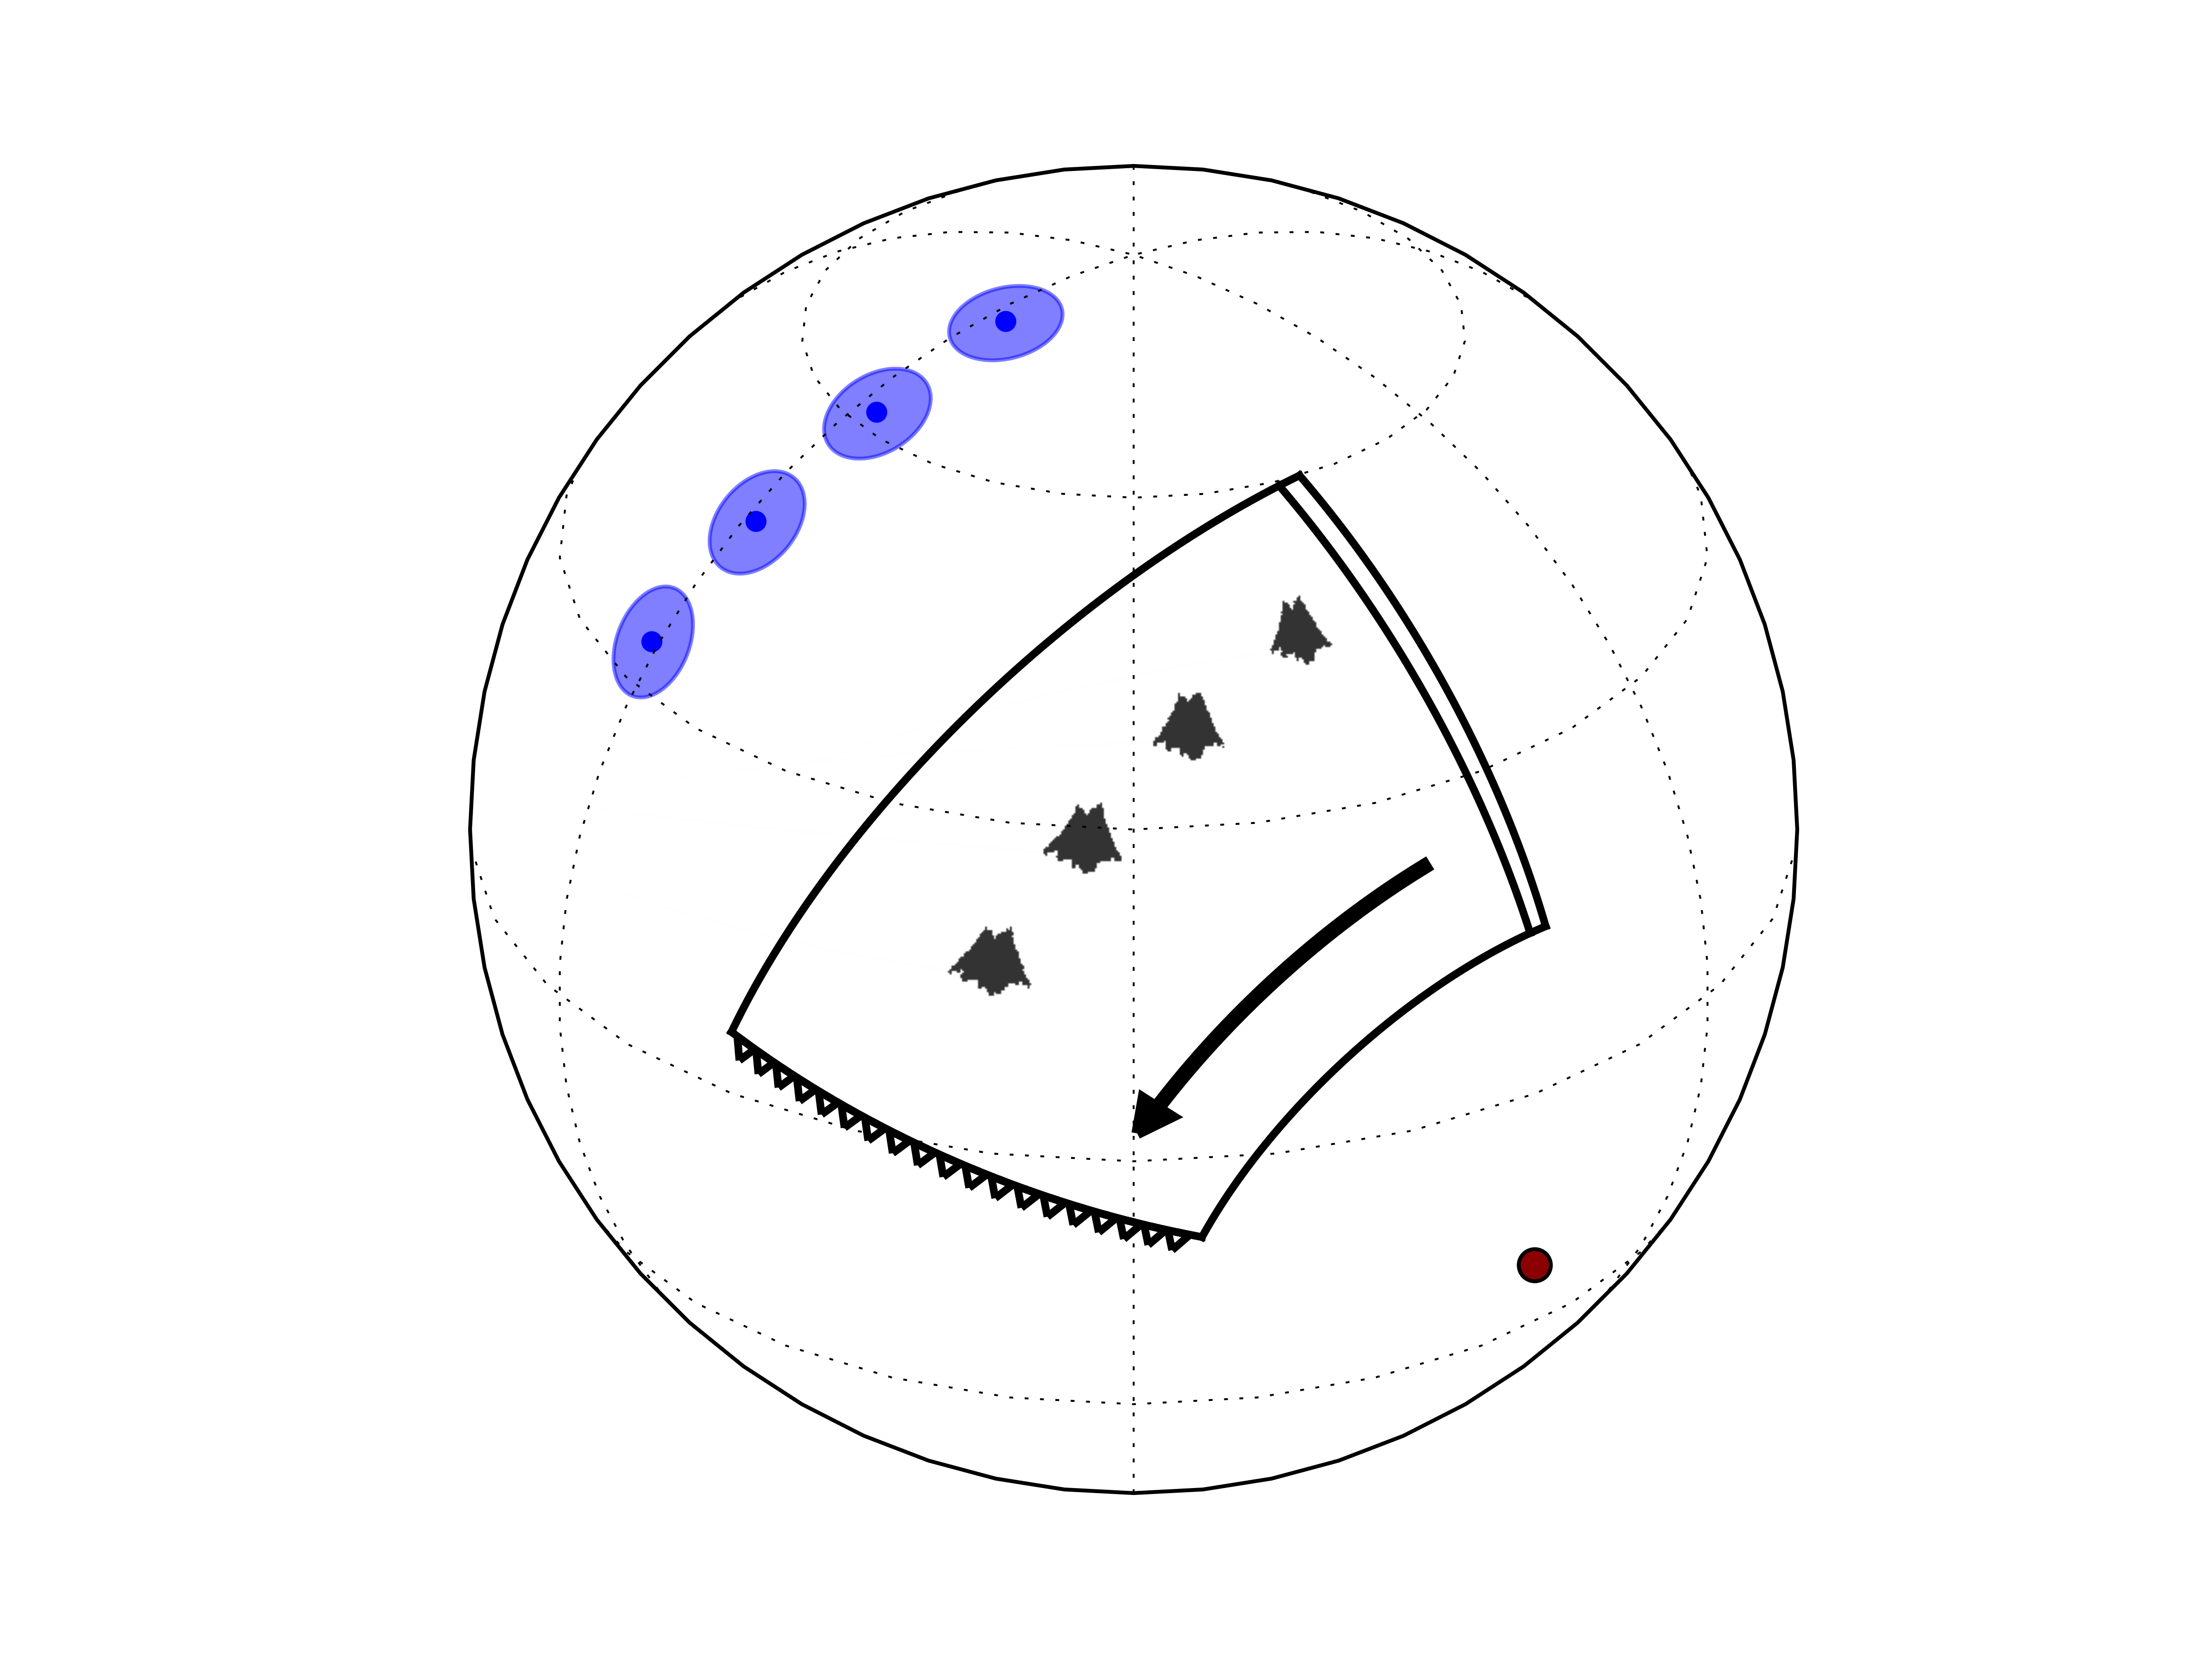
\includegraphics[width=0.9\textwidth]{figures/cartoon/paleomagnetic_euler_pole.png}
\caption[Conceptual model for a paleomagnetic Euler pole.]{Conceptual model for a paleomagnetic Euler pole. A finite rotation of the plate around an Euler pole results in long, arcuate oceanic fracture zones and hotspot tracks which describe small circles on the globe. The same finite rotation produces a small circle in the APW path. By fitting a small circle to the APW path we may recover the Euler pole that produced the rotation.}
\label{fig:pep}
\end{figure*}
A sequence of paleomagnetic poles from the same contintental block form an APW path,
which can then be analyzed to inform plate tectonic reconstructions and dynamic models
of plate speeds through time. 

\subsection{Latitudinal drift}
Due to the rotational symmetry of Earth's magnetic field, paleomagnetic poles do not
directly constrain the paleolongitude of the continental block in question \citep{butler1992paleomagnetism}.
The simplest analysis of an APW path is thus to compare the paleolatitudes of successive poles.
The difference in paleolatitudes gives a mininimum distance over which the block has traveled, 
corresponding to the great circle path between the two poles. If the two poles are well-dated,
this also furnishes a minimum rate of latitudinal motion.

It is also possible to fit
\subsection{Running means}

\subsection{Spherical splines}
\subsection{Paleomagnetic Euler poles}
\citet{gordon1984paleomagnetic}

\section{Bayesian inversion}
\label{sec:bayesian_inversion}
\subsection{A general desciption of inverse problems}
\label{sec:intro_inverse_problems}
The central question motivating inverse problems is ``How probable is a particular model, given my observations?''.
We represent a vector of individual observation by the data vector $\mathbf{d}$, and a model
by the vector of model parameters $\mathbf{m}$, so the above question can be written expressed as the function $P(\mathbf{m} \vert \mathbf{d})$.
Traditional frequentist approaches to an inverse problem often proceed by maximizing the likelihood function,
defined by the probability of the data given a particular model:
\begin{equation}
\mathcal{L} ( \mathbf{m} \vert \mathbf{d} ) = P( \mathbf{d} \vert \mathbf{m} ).
\label{eq:likelihood}
\end{equation}
The likelihood function replaces something that is difficult to compute ($P(\mathbf{m} \vert \mathbf{d})$)
with something that is less difficult to compute. 
To compute $\mathcal{L}(\mathbf{m}, \mathbf{d})$ we need to have two things: a statistical model for 
uncertainties in the observations $\mathbf{d}$ and forward model that allows us to compute
predictions ($\mathbf{d}_p$ of the observations from the model parameters, denoted by $\mathbf{g}$:
\begin{equation}
\mathbf{d}_p = \mathbf{g}(\mathbf{m}).
\label{eq:forward}
\end{equation}
For example, if each of the observed data $d_i$ are described with Gaussian uncertainties
with standard deviations $\sigma_i$, the likelihood function is given by the product
of the individual likelihoods of the observations:
\begin{equation}
\mathcal{L}(\mathbf{d} | \mathbf{m} ) = \displaystyle\prod_i \exp\left({-\frac{(d_i - d_{p,i})^2}{2 \sigma_i^2}}\right)
\label{eq:example_likelihood}
\end{equation}
The likelihood function $\mathcal{L}$ is maximized by searching over the model parameter space.
If the uncertainties in the observations are Gaussian, then maximizing the likelihood function is
equivalent to the least squares solution \citep{aster2005parameter}.

Frequently an unomdified maximum likelihood fit will overfit the observations, resulting
in unrealistic solutions. In the context of APW paths, these overfit solutions may
pass through every paleomagnetic pole, including less reliable ones, resulting in
loopy, sinuous paths. In order to address this, some form of regularization is usually
included in the solution of the inverse problem, such as penalizing the magnitude or
curvature of the solution. Both the running-mean and the spline under tension approaches
to APW paths can be seen as a form of regularization on the problem.

\subsection{Bayesian approach}

The Bayesian approach to inverse problems takes a different strategy from the frequentist one.
Rather than finding point estimates of a model fit, it treats the underlying model
as a set of random variables with individual probability distributions.
The probability distribution of the model $P(\mathbf{m} \vert \mathbf{d})$ 
is then found by an application of Bayes theorem:
\begin{equation}
P\left(\mathbf{m} \vert \mathbf{d} \right) = \frac{ P \left(\mathbf{d}\vert \mathbf{m} \right) P \left( \mathbf{m} \right) }{P \left( \mathbf{d}\right)}
\label{eq:bayes}
\end{equation}
It is often unnecessary to calculate the denominator of Equation~\eqref{eq:bayes}, leaving
\begin{equation}
P\left(\mathbf{m} \vert \mathbf{d} \right) \propto P \left( \mathbf{d} \vert \mathbf{m} \right) P \left( \mathbf{m} \right) 
\label{eq:propbayes}
\end{equation}
The quantity $P(\mathbf{m} \vert | \mathbf{d})$ is known as the posterior probability,
and represents our desired knowledge about the distributions of the paramters $\mathbf{m}$.
The first factor on the left-hand-side of Equation~\eqref{eq:propbayes} is identical to the likelihood
function described in Section~\ref{sec:intro_inverse_problems}, and the second factor
is known as the prior probability.

The inclusion of the prior probability allows us to incorporate additional knowledge
and beliefs about our inverse problem that is not otherwise included in the model.

\subsection{Markov chain Monte Carlo methods}


\subsection{Distributions on a sphere}

In order to proceed with a Bayesian description of the problem, every parameter
in the model should be described by some statistical distribution that determines
the probability that the parameter takes a specific value.
In addition to several more familiar 1D distributions (such as uniform or normal distributions)
we will also need to describe the statistics of points on a sphere, which we 
review here.


\subsubsection{Uniform distribution}
\begin{figure*}
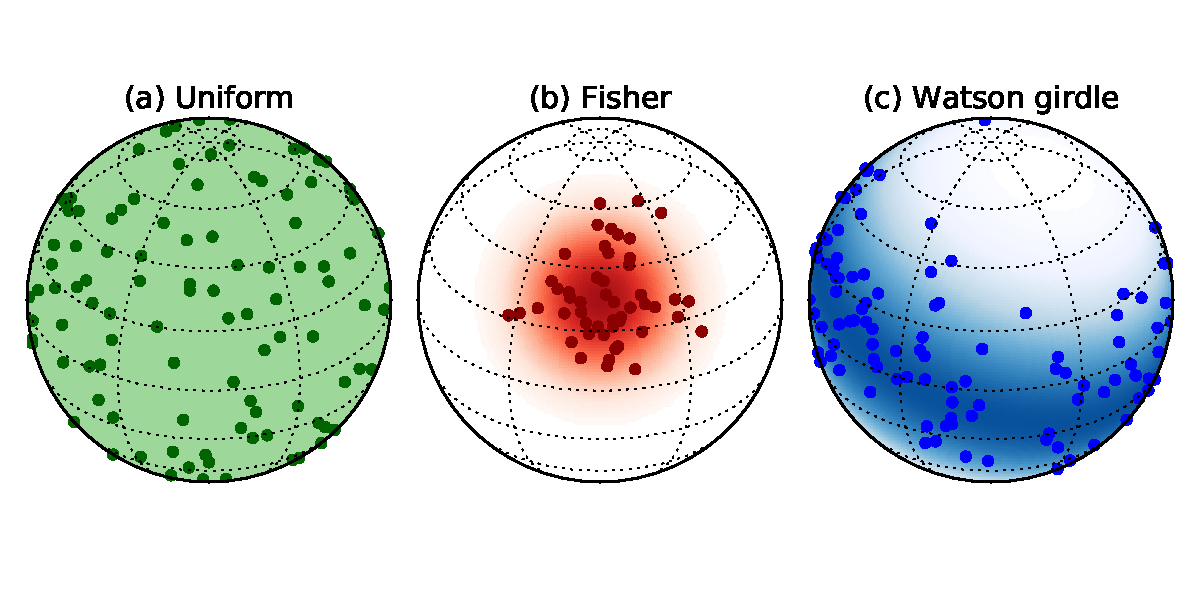
\includegraphics[width=0.9\textwidth]{figures/cartoon/distributions.pdf}
\caption[Spherical probability distributions.]{Probability densities for spherical distributions, as well as samples drawn from them. All are plotted using an orthographic projection. (a) Uniform distribution. (b) Fisher distribution. The center of the distribution is at $30^\circ$N, $30^\circ$E, and the concentration parameter $\kappa=20$. (c) Watson girdle distribution. The pole of symmetry is at $70^\circ$N, $90^\circ$E, and the concentration parameter $\kappa=-5$.}
\label{fig:distributions}
\end{figure*}

The simplest probability distribution on a sphere is the spherical uniform distribution, shown in Figure~\ref{fig:distributions}a.
It has a probability density given by
\begin{equation}
  \rho_U(\phi, \psi) = \frac{1}{4 \pi},
\end{equation}
where $\rho_U$ is the probability density, $\phi$ is the longitude, and $\psi$ is the latitude.
Most non-uniform distributions on a sphere reduce to the uniform distribution in some limit.
We will use this distribution when we want to specify an uninformative prior for directional parameters.

\subsubsection{Fisher distribution}
The Fisher distribution (also called the von Mises-Fisher distribution) is the analogue
of a 2D normal distribution on a sphere (see Figure~\ref{fig:fisher}).
The probability density $\rho_F$ for a unit vector $\hat{\mathbf{x}}$ is given by
\begin{equation}
  \begin{aligned}
  \rho_F(\phi, \psi ; \kappa_F, \hat{\mitbf{\mu}}) 
  &= \frac{1}{C_F} \exp \left( \kappa_F \hat{\mathbf{x}}^T \hat{\mitbf{\mu}} \right) \\
  &= \frac{1}{C_F} \exp \left( \kappa_F \cos \theta \right),
  \end{aligned}
\end{equation}
where $\kappa$ is the concentration of the distribution, 
$\hat{\mitbf{\mu}}$ the unit vector of the mean of the distribution, 
and $C_F$ is a normalization coefficient. It can be alternatively
parameterized using $\theta$, which is the angle between $\hat{\mathbf{x}}$ and $\hat{\mitbf{\mu}}$.
The normalization factor is given by 
\begin{equation}
  C_F = \frac{\kappa_F}{4 \pi \sinh{\kappa}}.
\end{equation}
The position and uncertainty of most paleomagnetic poles are represented by Fisher distributions,
and so we will use it to calculate the likelihood function of the model.

\subsubsection{Watson girdle distribution}
\begin{equation}
  \begin{aligned}
  \rho_W(\phi, \psi; \kappa_W, \hat{\mitbf{\mu}}) 
  &= \frac{1}{C_W} \exp \left( \kappa_W (\hat{\mathbf{x}}^T \hat{\mitbf{\mu}})^2 \right) \\
  &= \frac{1}{C_W} \exp \left( \kappa_W \cos^2 \theta \right)
  \end{aligned}
\end{equation}
\begin{equation}
  C_W = \left[ {}_1 F_1 \left( \frac{1}{2}, \frac{3}{2}, \kappa_W \right) \right]^{-1}
\end{equation}


\section{A model for PEP inversion}
\label{sec:model}
\subsection{Forward model}
\label{sec:forward_model}
The forward model for PEP analysis is essentially unchanged from that of \citet{gordon1984paleomagnetic}.
We describe plate motions (and hence paleomagnetic pole motions) with a series of Euler poles.
Each Euler pole has three parameters for which we are inverting (a latitude, a longitude and a rotation rate).

We furthermore need a set of changepoints, which denote the ages where we transition from 
one Euler pole to the next (the cusps, or ``hairpins'' of \citet{irving1972hairpins}).

Finally, we need a starting position on the globe, which, in practice, can be sampled
from the Fisher distribution of the oldest paleomagnetic pole in the dataset.
The starting point contributes two parameters (a latitude and a longitude).

All together, this means that for an inversion with $n_e$ Euler poles, 
the number parameters for which we are inverting is given by
\begin{equation}
\begin{aligned}
N &= 3 n_e + (n_e -1) + 2 \\
 &= 4 n_e + 1
\end{aligned}
\label{eq:n_parameters}
\end{equation}

For each Euler pole $\mitbf{\omega}_i$ the velocity $\mathbf{v}$ of a point 
$\mathbf{p}$ on the surface of the globe is given by
\begin{equation}
\mathbf{v} = \mitbf{\omega}_i \times \mathbf{p}.
\label{eq:rigid_rotation}
\end{equation}
Finite rotations can be performed by constructing Euler angle rotation matrices \citep[cf.][]{goldstein1965classical}. 
We generate synthetic paleomagnetic pole positions from the forward model by stringing together
finite rotations through the stage poles until the age of the paleomagnetic pole
is reached. These positions can then be compared to the actual paleomagnetic poles in our dataset.

\subsection{Choice of priors}

Bayesian analysis requires us to specify prior distributions for each of the parameters going into the inverse problem.
These distributions reflect our state of belief about the values of the parameters before we begin,
and allow us the option of incorporating information otherwise not captured by the model.
Typically we want to avoid biasing the results of the model towards a specific posterior distribution,
so we try to choose as uninformative a prior as possible. Depending upon the context, and the type
of parameter, that choice may vary.

The central parameters in the paleomagnetic Euler pole problem are the Euler pole positions,
the Euler pole magnitudes, the changepoints, and the starting point. 
The least informative prior for the i'th Euler pole is a uniform spherical distribution:
\begin{equation}
\hat{\mitbf{\omega}}_i \sim \rho_U(\phi, \psi)
\end{equation}
essentially allowing the Euler pole to be anywhere on the globe with equal probability.

The magnitude of each Euler pole is a strictly positive number, specifying the
rotation rate of that pole. In order to not bias the inversion towards a particular
rate we choose a uniform prior with large support. For the inversions shown in
this manuscript we use
\begin{equation}
\vert \mitbf{\omega}_i \vert \sim U(0, 10)
\end{equation}
where $U(\cdot, \cdot)$ is a uniform distribution between two values, and is given
in degrees per Myr. Typical rotation rates for present day plate motions
are around $1^\circ$/Myr \citep{argus2011geologically}.

The changepoints between successive Euler rotations should happen in the age
range specified by the oldest (at age $a_\mathrm{max}$) and youngest (at age $a_\mathrm{min}$)
paleomagnetic poles. We choose a uniform distribution as a prior for these changepoints:
\begin{equation}
c_i \sim U( a_\mathrm{min}, a_\mathrm{max}),
\end{equation}
where $c_i$ is the i'th changepoint.

Finally, the starting position $\hat{\mathbf{x}}_\mathrm{start}$ for the set of Euler pole rotations needs a prior.
We could choose another uniform distribution, but a more reasonable choice
is to start from near the oldest paleomagnetic pole in the dataset.
We therefore choose the Fisher distribution of the oldest paleomagnetic pole as a reasonable prior for a start point:
\begin{equation}
\hat{\mathbf{x}}_\mathrm{start} \sim \rho_F(\phi, \psi; \kappa_{F0}, \hat{\mitbf{\mu_0}})
\end{equation}
where $\kappa_{F0}$ and $\hat{\mitbf{\mu}}_0$ are the concentration parameter and mean direction
of the oldest paleomagnetic pole in the dataset.

One of the major advantages of Bayesian analysis is the ability to naturally incorporate
uncertainties in as many parameters as we need. A drawback of previous approaches
for modelling APWPs is that they do not easily account for uncertainties in
the age of paleomagnetic poles. In our approach we can include age uncertainty
by simply including the age of the poles as parameters in our model.

There are many different ways to constrain the ages of the geologic units from
which we obtain paleomagnetic poles, including radiometric dating, biostratigraphy,
magnetostratigraphy, cross-cutting relations, and stratigraphic relations.
Here we concentrate on just radiometric dating and stratigraphic constraints.
If a geologic unit has been radiometrically dated, we can model the age of
the j'th paleomagnetic pole $a_j$ as a normal distribution with mean $\mu_j$ and standard deviation $\sigma_j$:
\begin{equation}
a_j \sim N(\mu_j, \sigma_j)
\end{equation}
where $N(.,.)$ denotes a normal distribution.

Freqently, however, the geologic unit from which we obtain a paleomagnetic pole
is not well dated, and its age can only be constrained to lie between those
of well-dated units stratigraphically above and below it. In this case,
we argue that a uniform distribution between those ages is a reasonable choice
of prior:
\begin{equation}
a_j \sim U(a_\mathrm{low}, a_\mathrm{high})
\end{equation}
where $a_\mathrm{low}$ and $a_\mathrm{high}$ are the ages of the upper and lower
well-dated stratigraphic units, respectively.

To summarize our choices for priors:
\begin{itemize}
\item Euler pole positions: spherical uniform distribution.
\item Euler pole magnitudes: Uniform distribution between 0$^\circ$ and 10$^\circ$/Myr.
\item Changepoints: uniform distribution between $a_\mathrm{min}$ and $a_\mathrm{max}$.
\item Paleomagnetic pole ages: normal or uniform distribution, depending on the type of age control for the geologic unit.
\end{itemize}


INCLUDE DISCUSSION OF WATSON PRIOR ON EULER POLES?


\subsection{Likelihood}

In addition to the choice of priors, we also need a statistical description of the observations.
This will allow us to calculate the likelihood function, which, when combined with the priors,
allows us to evaluate Bayes' theorem (Equation~\eqref{eq:propbayes}).

In the case of APW paths, our observations are paleomagnetic poles.
The most common statistical distribution for describing paleomagnetic poles is the Fisher distribution
(though others are possible, such as the Kent or Bingham distribitions, c.f. \citet{tauxe2009essentials}).
Given the set of model parameters $\mathbf{m}$ and the forward model $\mathbf{g}(\mathbf{m})$, described
in Section~\ref{sec:forward_model}, we can calculate the predicted paleomagnetic pole unit vectors $\hat{\mathbf{x}}_{p,i}$.
For a set of $i$ paleomagnetic poles, the likelihood is then given by the product of the probabilities
of each observation:
\begin{equation}
P(\mathbf{d} \vert \mathbf{m}) = \displaystyle\prod_i \frac{1}{C_{F,i}} \exp \left( \kappa_{F,i} \hat{\mathbf{x}}_{p,i}^T \hat{\mitbf{\mu}}_i \right).
\label{eq:model_likelihood}
\end{equation}


\subsection{Model selection}

\section{Example inversions}
\label{sec:example_inversion}

Before proceeding with inversions for paleomagnetic Euler poles using real paleomagnetic data,
it is useful to consider a few examples of inversions for synthetic datasets.

We begin by trying to recover the Euler pole for a single rotation.
We generate a synthetic APW track of four poles

\subsection{One stage pole}

\begin{figure*}
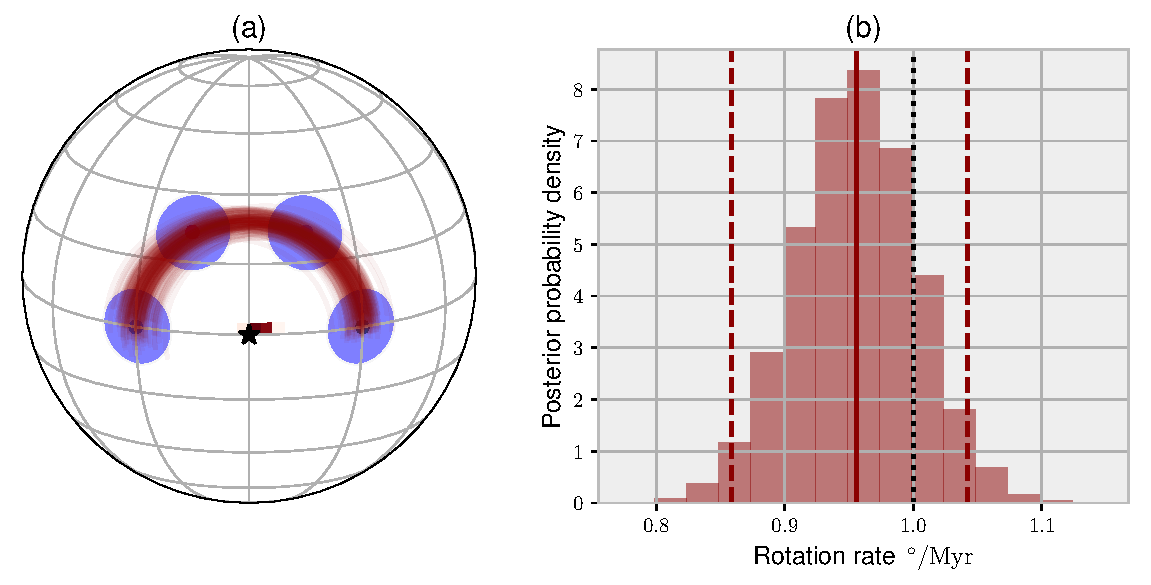
\includegraphics[width=0.9\textwidth]{figures/synthetic/one_euler_pole.pdf}
\caption[Inversion for a single paleomagnetic Euler pole.]{Inversion for a single paleomagnetic Euler pole (PEP). (a) Four paleomagnetic poles are generated during a net $180^\circ$ rotation about an Euler pole at $0^\circ$N, $0^\circ$E over 30 Myr, for a rotation rate of $6^\circ$/Myr. The red distribution is the probability density function recovered by MCMC inversion, and the red lines are a sampling of the synthetic APW paths generated by the inversion. (b) Posterior probability density for the rotation rate of the Euler pole recovered by the inversion. The peak of the distribution slightly underestimates the true value of $6^\circ$/Myr, and the great majority of the probability lies between $4^\circ-7^\circ$/Myr. }
\label{fig:one_euler_pole}
\end{figure*}

\subsection{Two stage poles}
\begin{figure*}
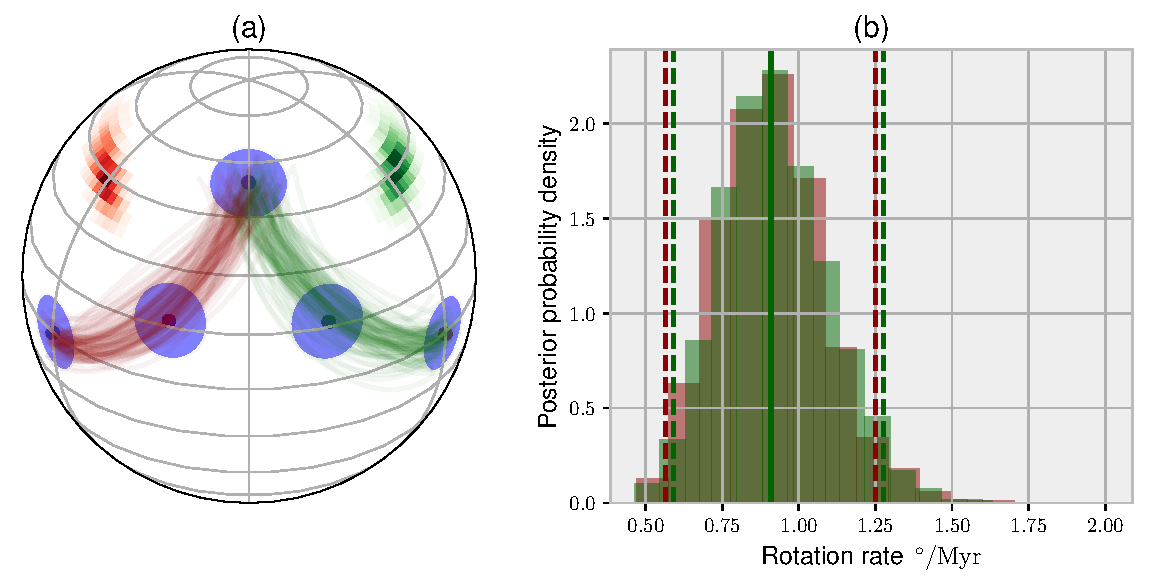
\includegraphics[width=0.9\textwidth]{figures/synthetic/two_euler_poles.pdf}
\caption[Inversion for two successive paleomagnetic Euler poles.]{Inversion for two successive paleomagnetic Euler poles. (a) Five paleomagnetic poles are generated, beginning with a pole at $0^\circ$N, $60^\circ$W. The first Euler pole is located at $41^\circ$N, $60^\circ$W, and rotates at $6.5^\circ$/Myr for 20 Myr. The second Euler pole is located at $41^\circ$N, $60^\circ$W, and rotates at the same speed and for the same duration. The red and green distributions show the location of the first and second Euler poles (respectively) recovered by the MCMC inversion. The the red and green lines are a sampling of the synthetic APW paths generated by the inversion. (b) Posterior probability density for the rotation rates of the Euler poles recovered by the inversion.}
\label{fig:two_euler_poles}
\end{figure*}
\subsection{Incorporating age uncertainty}
\begin{figure*}
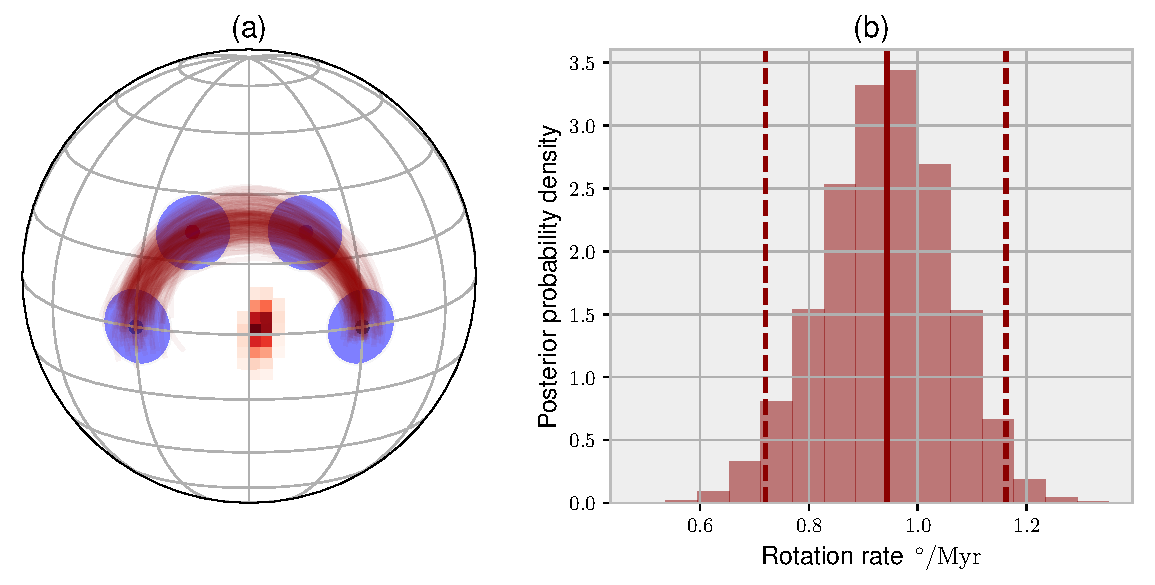
\includegraphics[width=0.9\textwidth]{figures/synthetic/age_uncertainty.pdf}
\caption[Inversion for a paleomagnetic Euler pole, incorporating age uncertainty.]{Inversion for a single paleomagnetic Euler pole, but including uncertainty in the ages. (a) Four paleomagnetic poles are generated by a $180^\circ$ rotation about an Euler pole at $0^\circ$N, $0^\circ$E over 30 Myr, for a rotation rate of $6^\circ$/Myr (same as the ``One stage pole'' example). The red distribution is the probability density function recovered by MCMC inversion, and the red lines are a sampling of the synthetic APW paths generated by the inversion. (b) Posterior probability density for the rotation rate of the Euler pole recovered by the inversion.}
\label{fig:age_uncertainty}
\end{figure*}
\begin{figure*}
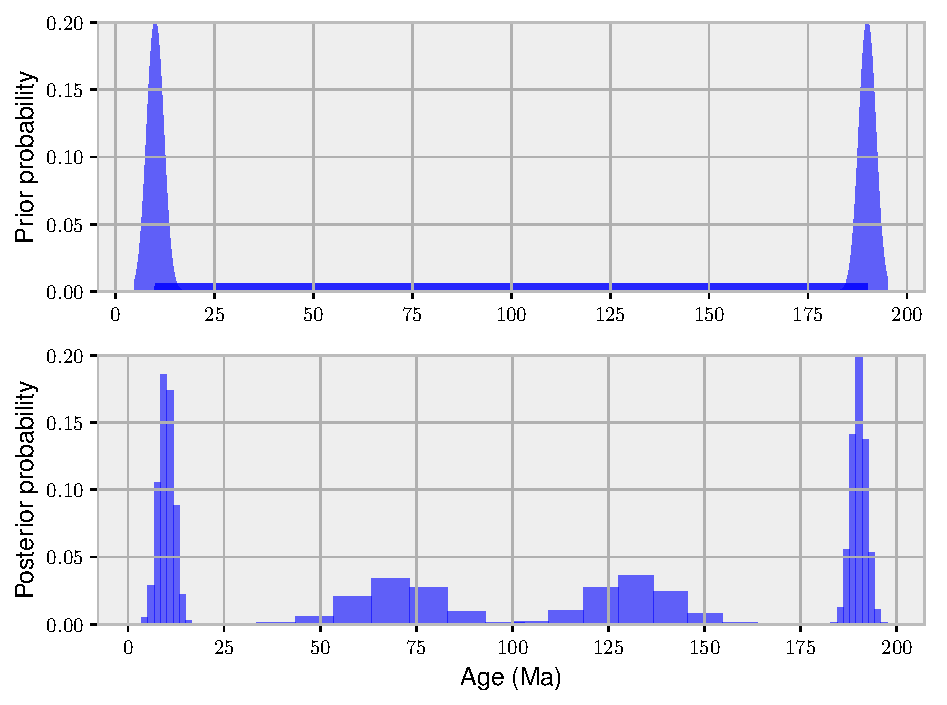
\includegraphics[width=0.9\textwidth]{figures/synthetic/age_uncertainty_samples.pdf}
\caption{}
\label{fig:age_uncertainty_samples}
\end{figure*}

\section{Application to Cenozoic Australian APW path}
\label{sec:australia}
\clearpage
\begin{figure*}
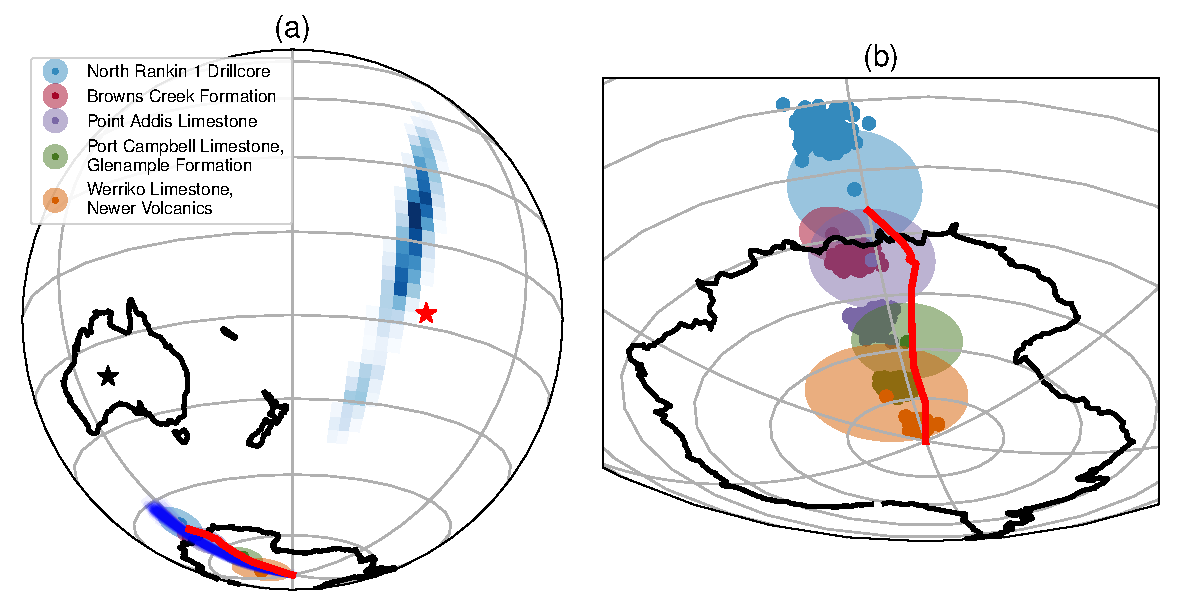
\includegraphics[width=0.9\textwidth]{figures/australia/australia_paths_1.pdf}
\caption{}
\label{fig:australia_paths_1}
\end{figure*}
\begin{figure*}
\includegraphics[width=0.9\textwidth]{figures/australia/australia_latitude_1.pdf}
\caption{}
\label{fig:australia_latitude_1}
\end{figure*}
\begin{figure*}
\includegraphics[width=0.9\textwidth]{figures/australia/australia_ages_1.pdf}
\caption{}
\label{fig:australia_ages_1}
\end{figure*}
\begin{figure*}
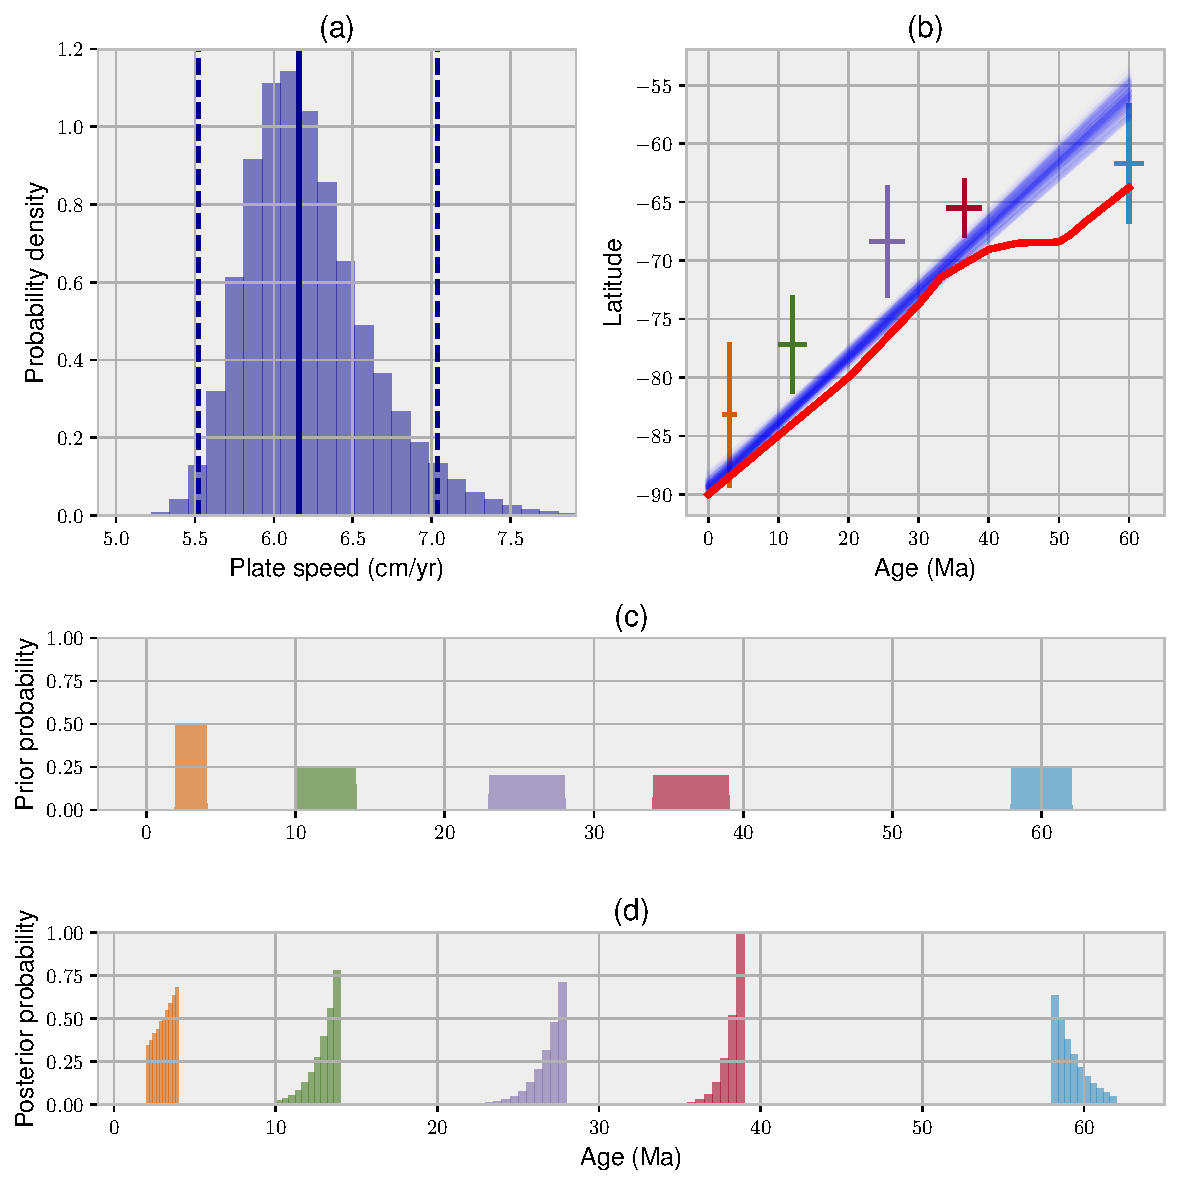
\includegraphics[width=0.9\textwidth]{figures/australia/australia_speeds_1.pdf}
\caption{}
\label{fig:australia_speeds_1}
\end{figure*}
\begin{figure*}
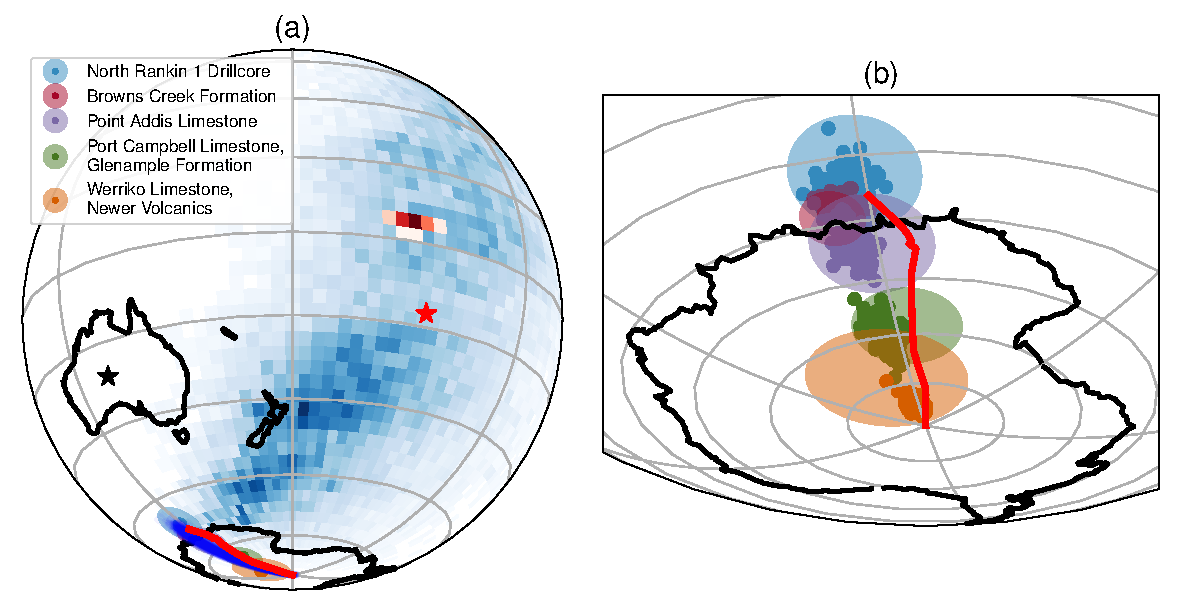
\includegraphics[width=0.9\textwidth]{figures/australia/australia_paths_2.pdf}
\caption{}
\label{fig:australia_paths_2}
\end{figure*}
\begin{figure*}
\includegraphics[width=0.9\textwidth]{figures/australia/australia_ages_2.pdf}
\caption{}
\label{fig:australia_ages_2}
\end{figure*}
\begin{figure*}
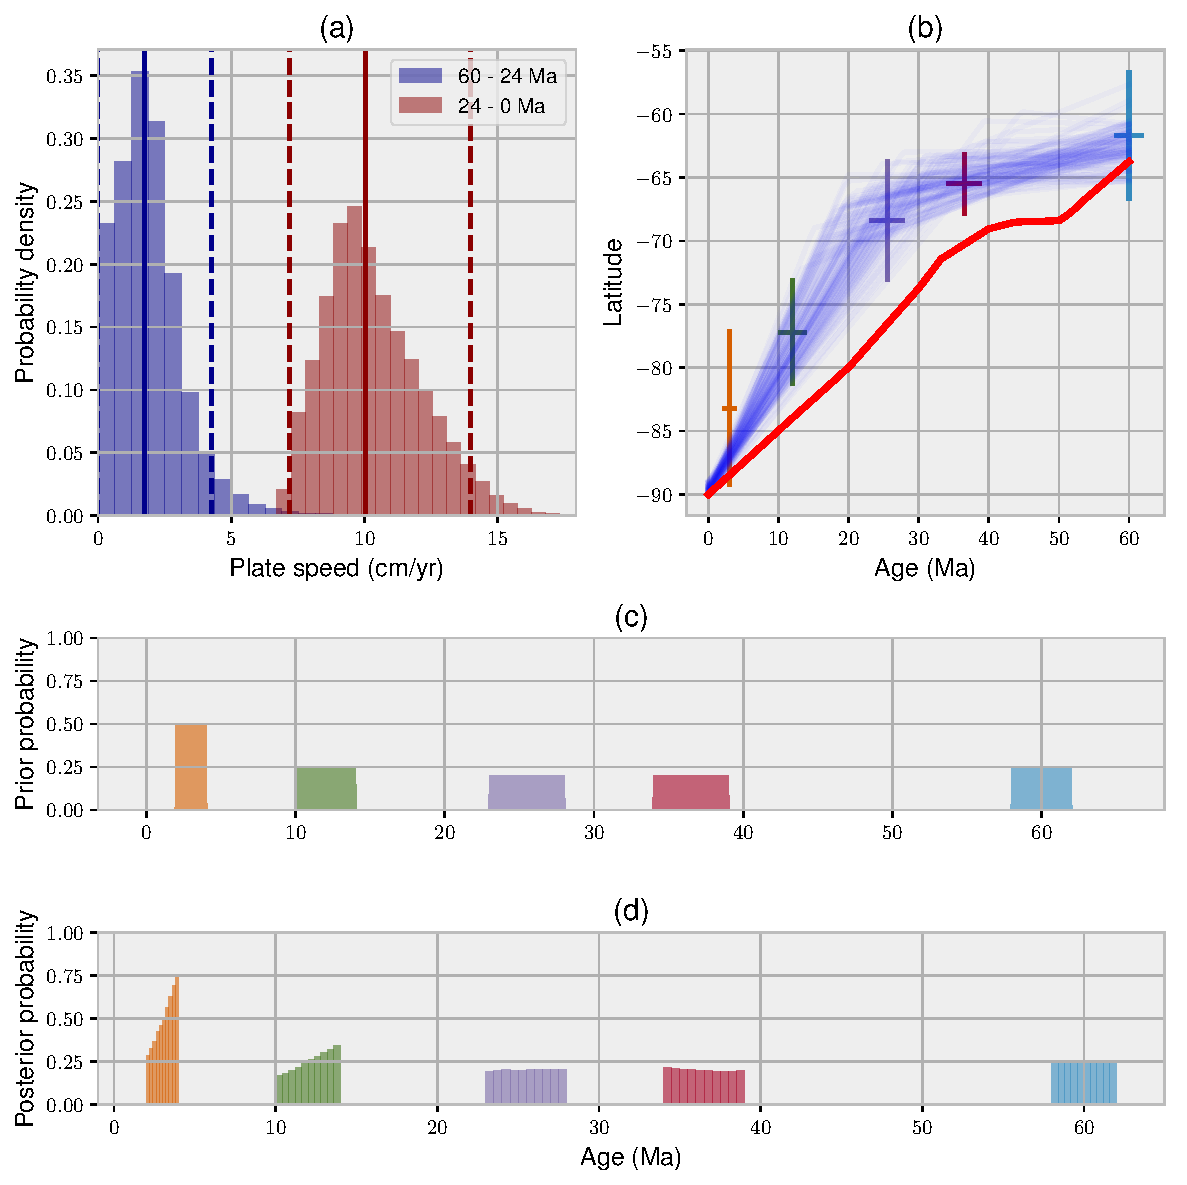
\includegraphics[width=0.9\textwidth]{figures/australia/australia_speeds_2.pdf}
\caption{}
\label{fig:australia_speeds_2}
\end{figure*}
\begin{figure*}
\includegraphics[width=0.9\textwidth]{figures/australia/australia_latitude_2.pdf}
\caption{}
\label{fig:australia_latitude_2}
\end{figure*}


\section{Application to the Keweenawan province}
\label{sec:keweenawan}
\subsection{Geologic context}
\citet{swanson2009no}
\subsection{Inversion for paleomagnetic Euler poles}
\clearpage
\begin{figure*}
\includegraphics[width=0.9\textwidth]{figures/keweenawan/keweenawan_paths_1.pdf}
\caption{}
\label{fig:keweenawan_paths_1}
\end{figure*}
\begin{figure*}
\includegraphics[width=0.9\textwidth]{figures/keweenawan/keweenawan_ages_1.pdf}
\caption{}
\label{fig:keweenawan_ages_1}
\end{figure*}
\begin{figure*}
\includegraphics[width=0.9\textwidth]{figures/keweenawan/keweenawan_speeds_1.pdf}
\caption{}
\label{fig:keweenawan_speeds_1}
\end{figure*}
\begin{figure*}
\includegraphics[width=0.9\textwidth]{figures/keweenawan/keweenawan_paths_2.pdf}
\caption{}
\label{fig:keweenawan_paths_2}
\end{figure*}
\begin{figure*}
\includegraphics[width=0.9\textwidth]{figures/keweenawan/keweenawan_ages_2.pdf}
\caption{}
\label{fig:keweenawan_ages_2}
\end{figure*}
\begin{figure*}
\includegraphics[width=0.9\textwidth]{figures/keweenawan/keweenawan_speeds_2.pdf}
\caption{}
\label{fig:keweenawan_speeds_2}
\end{figure*}
\subsection{Plate speeds for Mesoproterozoic Laurentia}

\section{Conclusions}
\label{sec:conclusions}



%% The Appendices part is started with the command \appendix;
%% appendix sections are then done as normal sections
%% \appendix

%% \section{}
%% \label{}

%% If you have bibdatabase file and want bibtex to generate the
%% bibitems, please use
%%
\bibliographystyle{elsarticle-harv} 
\bibliography{bayesian_plate_reconstruction}

%% else use the following coding to input the bibitems directly in the
%% TeX file.

\end{document}

\endinput
%%
%% End of file `elsarticle-template-harv.tex'.
